% Options for packages loaded elsewhere
\PassOptionsToPackage{unicode}{hyperref}
\PassOptionsToPackage{hyphens}{url}
%
\documentclass[
]{article}
\usepackage{amsmath,amssymb}
\usepackage{iftex}
\ifPDFTeX
  \usepackage[T1]{fontenc}
  \usepackage[utf8]{inputenc}
  \usepackage{textcomp} % provide euro and other symbols
\else % if luatex or xetex
  \usepackage{unicode-math} % this also loads fontspec
  \defaultfontfeatures{Scale=MatchLowercase}
  \defaultfontfeatures[\rmfamily]{Ligatures=TeX,Scale=1}
\fi
\usepackage{lmodern}
\ifPDFTeX\else
  % xetex/luatex font selection
\fi
% Use upquote if available, for straight quotes in verbatim environments
\IfFileExists{upquote.sty}{\usepackage{upquote}}{}
\IfFileExists{microtype.sty}{% use microtype if available
  \usepackage[]{microtype}
  \UseMicrotypeSet[protrusion]{basicmath} % disable protrusion for tt fonts
}{}
\makeatletter
\@ifundefined{KOMAClassName}{% if non-KOMA class
  \IfFileExists{parskip.sty}{%
    \usepackage{parskip}
  }{% else
    \setlength{\parindent}{0pt}
    \setlength{\parskip}{6pt plus 2pt minus 1pt}}
}{% if KOMA class
  \KOMAoptions{parskip=half}}
\makeatother
\usepackage{xcolor}
\usepackage[margin=1in]{geometry}
\usepackage{color}
\usepackage{fancyvrb}
\newcommand{\VerbBar}{|}
\newcommand{\VERB}{\Verb[commandchars=\\\{\}]}
\DefineVerbatimEnvironment{Highlighting}{Verbatim}{commandchars=\\\{\}}
% Add ',fontsize=\small' for more characters per line
\usepackage{framed}
\definecolor{shadecolor}{RGB}{248,248,248}
\newenvironment{Shaded}{\begin{snugshade}}{\end{snugshade}}
\newcommand{\AlertTok}[1]{\textcolor[rgb]{0.94,0.16,0.16}{#1}}
\newcommand{\AnnotationTok}[1]{\textcolor[rgb]{0.56,0.35,0.01}{\textbf{\textit{#1}}}}
\newcommand{\AttributeTok}[1]{\textcolor[rgb]{0.13,0.29,0.53}{#1}}
\newcommand{\BaseNTok}[1]{\textcolor[rgb]{0.00,0.00,0.81}{#1}}
\newcommand{\BuiltInTok}[1]{#1}
\newcommand{\CharTok}[1]{\textcolor[rgb]{0.31,0.60,0.02}{#1}}
\newcommand{\CommentTok}[1]{\textcolor[rgb]{0.56,0.35,0.01}{\textit{#1}}}
\newcommand{\CommentVarTok}[1]{\textcolor[rgb]{0.56,0.35,0.01}{\textbf{\textit{#1}}}}
\newcommand{\ConstantTok}[1]{\textcolor[rgb]{0.56,0.35,0.01}{#1}}
\newcommand{\ControlFlowTok}[1]{\textcolor[rgb]{0.13,0.29,0.53}{\textbf{#1}}}
\newcommand{\DataTypeTok}[1]{\textcolor[rgb]{0.13,0.29,0.53}{#1}}
\newcommand{\DecValTok}[1]{\textcolor[rgb]{0.00,0.00,0.81}{#1}}
\newcommand{\DocumentationTok}[1]{\textcolor[rgb]{0.56,0.35,0.01}{\textbf{\textit{#1}}}}
\newcommand{\ErrorTok}[1]{\textcolor[rgb]{0.64,0.00,0.00}{\textbf{#1}}}
\newcommand{\ExtensionTok}[1]{#1}
\newcommand{\FloatTok}[1]{\textcolor[rgb]{0.00,0.00,0.81}{#1}}
\newcommand{\FunctionTok}[1]{\textcolor[rgb]{0.13,0.29,0.53}{\textbf{#1}}}
\newcommand{\ImportTok}[1]{#1}
\newcommand{\InformationTok}[1]{\textcolor[rgb]{0.56,0.35,0.01}{\textbf{\textit{#1}}}}
\newcommand{\KeywordTok}[1]{\textcolor[rgb]{0.13,0.29,0.53}{\textbf{#1}}}
\newcommand{\NormalTok}[1]{#1}
\newcommand{\OperatorTok}[1]{\textcolor[rgb]{0.81,0.36,0.00}{\textbf{#1}}}
\newcommand{\OtherTok}[1]{\textcolor[rgb]{0.56,0.35,0.01}{#1}}
\newcommand{\PreprocessorTok}[1]{\textcolor[rgb]{0.56,0.35,0.01}{\textit{#1}}}
\newcommand{\RegionMarkerTok}[1]{#1}
\newcommand{\SpecialCharTok}[1]{\textcolor[rgb]{0.81,0.36,0.00}{\textbf{#1}}}
\newcommand{\SpecialStringTok}[1]{\textcolor[rgb]{0.31,0.60,0.02}{#1}}
\newcommand{\StringTok}[1]{\textcolor[rgb]{0.31,0.60,0.02}{#1}}
\newcommand{\VariableTok}[1]{\textcolor[rgb]{0.00,0.00,0.00}{#1}}
\newcommand{\VerbatimStringTok}[1]{\textcolor[rgb]{0.31,0.60,0.02}{#1}}
\newcommand{\WarningTok}[1]{\textcolor[rgb]{0.56,0.35,0.01}{\textbf{\textit{#1}}}}
\usepackage{graphicx}
\makeatletter
\def\maxwidth{\ifdim\Gin@nat@width>\linewidth\linewidth\else\Gin@nat@width\fi}
\def\maxheight{\ifdim\Gin@nat@height>\textheight\textheight\else\Gin@nat@height\fi}
\makeatother
% Scale images if necessary, so that they will not overflow the page
% margins by default, and it is still possible to overwrite the defaults
% using explicit options in \includegraphics[width, height, ...]{}
\setkeys{Gin}{width=\maxwidth,height=\maxheight,keepaspectratio}
% Set default figure placement to htbp
\makeatletter
\def\fps@figure{htbp}
\makeatother
\setlength{\emergencystretch}{3em} % prevent overfull lines
\providecommand{\tightlist}{%
  \setlength{\itemsep}{0pt}\setlength{\parskip}{0pt}}
\setcounter{secnumdepth}{-\maxdimen} % remove section numbering
\ifLuaTeX
  \usepackage{selnolig}  % disable illegal ligatures
\fi
\usepackage{bookmark}
\IfFileExists{xurl.sty}{\usepackage{xurl}}{} % add URL line breaks if available
\urlstyle{same}
\hypersetup{
  pdftitle={p8130\_hw4\_xx2485},
  pdfauthor={Xiaoni Xu},
  hidelinks,
  pdfcreator={LaTeX via pandoc}}

\title{p8130\_hw4\_xx2485}
\author{Xiaoni Xu}
\date{2024-11-16}

\begin{document}
\maketitle

Loading needed packages

\begin{Shaded}
\begin{Highlighting}[]
\FunctionTok{library}\NormalTok{(readxl)}
\FunctionTok{library}\NormalTok{(janitor)}
\FunctionTok{library}\NormalTok{(tidyverse)}
\FunctionTok{library}\NormalTok{(knitr)}
\FunctionTok{library}\NormalTok{(ggplot2)}
\end{Highlighting}
\end{Shaded}

\subsection{Problem 1}\label{problem-1}

Perform sign test.

\begin{Shaded}
\begin{Highlighting}[]
\NormalTok{data }\OtherTok{\textless{}{-}} \FunctionTok{c}\NormalTok{(}\DecValTok{125}\NormalTok{, }\DecValTok{123}\NormalTok{, }\DecValTok{117}\NormalTok{, }\DecValTok{123}\NormalTok{, }\DecValTok{115}\NormalTok{, }\DecValTok{112}\NormalTok{, }\DecValTok{128}\NormalTok{, }\DecValTok{118}\NormalTok{, }\DecValTok{124}\NormalTok{, }\DecValTok{111}\NormalTok{, }\DecValTok{116}\NormalTok{, }\DecValTok{109}\NormalTok{, }
          \DecValTok{125}\NormalTok{, }\DecValTok{120}\NormalTok{, }\DecValTok{113}\NormalTok{, }\DecValTok{123}\NormalTok{, }\DecValTok{112}\NormalTok{, }\DecValTok{118}\NormalTok{, }\DecValTok{121}\NormalTok{, }\DecValTok{118}\NormalTok{, }\DecValTok{122}\NormalTok{, }\DecValTok{115}\NormalTok{, }\DecValTok{105}\NormalTok{, }\DecValTok{118}\NormalTok{, }\DecValTok{131}\NormalTok{)}

\CommentTok{\# Define the hypothesized median}
\NormalTok{median\_hypothesis }\OtherTok{\textless{}{-}} \DecValTok{120}

\CommentTok{\# Count values above and below the hypothesized median}
\NormalTok{above }\OtherTok{\textless{}{-}} \FunctionTok{sum}\NormalTok{(data }\SpecialCharTok{\textgreater{}}\NormalTok{ median\_hypothesis)}
\NormalTok{below }\OtherTok{\textless{}{-}} \FunctionTok{sum}\NormalTok{(data }\SpecialCharTok{\textless{}}\NormalTok{ median\_hypothesis)}

\CommentTok{\# Perform the sign test}
\NormalTok{binom\_test }\OtherTok{\textless{}{-}} \FunctionTok{binom.test}\NormalTok{(below, below }\SpecialCharTok{+}\NormalTok{ above, }\AttributeTok{p =} \FloatTok{0.5}\NormalTok{, }\AttributeTok{alternative =} \StringTok{"less"}\NormalTok{)}

\CommentTok{\# Report results}
\NormalTok{binom\_test}
\end{Highlighting}
\end{Shaded}

\begin{verbatim}
## 
##  Exact binomial test
## 
## data:  below and below + above
## number of successes = 14, number of trials = 24, p-value = 0.8463
## alternative hypothesis: true probability of success is less than 0.5
## 95 percent confidence interval:
##  0.0000000 0.7536114
## sample estimates:
## probability of success 
##              0.5833333
\end{verbatim}

We conducted an exact binomial test to evaluate whether the median blood
sugar level in the population is less than 120. The hypotheses were as
follows:

\[
H_0: \text{The true median is } \geq 120 \quad \text{(probability of success } = 0.5\text{)}.
\] \[
H_a: \text{The true median is } < 120 \quad \text{(probability of success } > 0.5\text{)}.
\]

The test results are: - Number of successes (blood sugar readings below
120): \(14\) - Number of trials: \(24\) - p-value: \(0.8463\) - 95\%
confidence interval for the probability of success: \([0.000, 0.7536]\)

Since the p-value (\(0.8463\)) is greater than the significance level
(\(\alpha = 0.05\)), we fail to reject the null hypothesis.

Conclusion: There is no statistically significant evidence to suggest
that the median blood sugar level in the population is less than 120.

The test statistic is 14.

Perform Wilcoxon signed-rank test.

\begin{Shaded}
\begin{Highlighting}[]
\CommentTok{\# Calculate differences from the hypothesized median}
\NormalTok{differences }\OtherTok{\textless{}{-}}\NormalTok{ data }\SpecialCharTok{{-}} \DecValTok{120}

\CommentTok{\# Remove zero differences}
\NormalTok{nonzero\_differences }\OtherTok{\textless{}{-}}\NormalTok{ differences[differences }\SpecialCharTok{!=} \DecValTok{0}\NormalTok{]}

\CommentTok{\# Rank absolute differences, handling ties with average ranks}
\NormalTok{abs\_differences }\OtherTok{\textless{}{-}} \FunctionTok{abs}\NormalTok{(nonzero\_differences)}
\NormalTok{ranks }\OtherTok{\textless{}{-}} \FunctionTok{rank}\NormalTok{(abs\_differences)}

\CommentTok{\# Sum ranks for negative differences}
\NormalTok{negative\_ranks }\OtherTok{\textless{}{-}}\NormalTok{ ranks[nonzero\_differences }\SpecialCharTok{\textless{}} \DecValTok{0}\NormalTok{]}
\NormalTok{W\_minus }\OtherTok{\textless{}{-}} \FunctionTok{sum}\NormalTok{(negative\_ranks)}

\CommentTok{\# Calculate p{-}value using the normal approximation}
\NormalTok{n }\OtherTok{\textless{}{-}} \FunctionTok{length}\NormalTok{(nonzero\_differences)}
\NormalTok{mean\_W }\OtherTok{\textless{}{-}}\NormalTok{ n }\SpecialCharTok{*}\NormalTok{ (n }\SpecialCharTok{+} \DecValTok{1}\NormalTok{) }\SpecialCharTok{/} \DecValTok{4}
\NormalTok{sd\_W }\OtherTok{\textless{}{-}} \FunctionTok{sqrt}\NormalTok{(n }\SpecialCharTok{*}\NormalTok{ (n }\SpecialCharTok{+} \DecValTok{1}\NormalTok{) }\SpecialCharTok{*}\NormalTok{ (}\DecValTok{2} \SpecialCharTok{*}\NormalTok{ n }\SpecialCharTok{+} \DecValTok{1}\NormalTok{) }\SpecialCharTok{/} \DecValTok{24}\NormalTok{)}

\NormalTok{z }\OtherTok{\textless{}{-}}\NormalTok{ (W\_minus }\SpecialCharTok{{-}}\NormalTok{ mean\_W) }\SpecialCharTok{/}\NormalTok{ sd\_W}
\NormalTok{p\_value }\OtherTok{\textless{}{-}} \FunctionTok{pnorm}\NormalTok{(z)}

\CommentTok{\# Results}
\FunctionTok{list}\NormalTok{(}
  \AttributeTok{test\_statistic =}\NormalTok{ W\_minus,}
  \AttributeTok{p\_value =}\NormalTok{ p\_value,}
  \AttributeTok{z\_score =}\NormalTok{ z}
\NormalTok{)}
\end{Highlighting}
\end{Shaded}

\begin{verbatim}
## $test_statistic
## [1] 187.5
## 
## $p_value
## [1] 0.8580116
## 
## $z_score
## [1] 1.071429
\end{verbatim}

Since the p-value (\(0.8580\)) is greater than the significance level
(\(\alpha = 0.05\)), we fail to reject the null hypothesis.

There is no statistically significant evidence to suggest that the
median blood sugar level in the population is less than 120.

\subsection{Problem 2}\label{problem-2}

\subsubsection{(a)}\label{a}

\begin{Shaded}
\begin{Highlighting}[]
\CommentTok{\# Load the data}
\NormalTok{brain }\OtherTok{\textless{}{-}} \FunctionTok{read\_excel}\NormalTok{(}\StringTok{"Brain.xlsx"}\NormalTok{) }\SpecialCharTok{\%\textgreater{}\%} 
  \FunctionTok{clean\_names}\NormalTok{()}


\CommentTok{\# Filter out the human species (Homo sapiens)}
\NormalTok{nonhuman\_data }\OtherTok{\textless{}{-}} \FunctionTok{subset}\NormalTok{(brain, species }\SpecialCharTok{!=} \StringTok{"Homo sapiens"}\NormalTok{)}

\CommentTok{\# Fit a regression model using ln\_brain\_mass as the predictor for glia\_neuron\_ratio}
\NormalTok{model }\OtherTok{\textless{}{-}} \FunctionTok{lm}\NormalTok{(glia\_neuron\_ratio }\SpecialCharTok{\textasciitilde{}}\NormalTok{ ln\_brain\_mass, }\AttributeTok{data =}\NormalTok{ nonhuman\_data)}

\CommentTok{\# Summary of the regression model}
\FunctionTok{summary}\NormalTok{(model)}
\end{Highlighting}
\end{Shaded}

\begin{verbatim}
## 
## Call:
## lm(formula = glia_neuron_ratio ~ ln_brain_mass, data = nonhuman_data)
## 
## Residuals:
##      Min       1Q   Median       3Q      Max 
## -0.24150 -0.12030 -0.01787  0.15940  0.25563 
## 
## Coefficients:
##               Estimate Std. Error t value Pr(>|t|)    
## (Intercept)    0.16370    0.15987   1.024 0.322093    
## ln_brain_mass  0.18113    0.03604   5.026 0.000151 ***
## ---
## Signif. codes:  0 '***' 0.001 '**' 0.01 '*' 0.05 '.' 0.1 ' ' 1
## 
## Residual standard error: 0.1699 on 15 degrees of freedom
## Multiple R-squared:  0.6274, Adjusted R-squared:  0.6025 
## F-statistic: 25.26 on 1 and 15 DF,  p-value: 0.0001507
\end{verbatim}

The regression model shows that \(\ln(\text{Brain Mass})\) is a
significant predictor of the glia-neuron ratio in nonhuman species
(\(p < 0.001\)). The positive slope (\(0.1811\)) indicates that species
with larger brain masses (in terms of the natural logarithm) tend to
have higher glia-neuron ratios. The model explains a substantial portion
of the variability in the data (\(R^2 = 0.6274\)), making it a good fit
for the observed relationship.

\subsubsection{(b)}\label{b}

\begin{Shaded}
\begin{Highlighting}[]
\CommentTok{\# Given human brain mass}
\NormalTok{human\_brain\_mass }\OtherTok{\textless{}{-}} \FloatTok{1373.3}

\CommentTok{\# Calculate the natural logarithm of human brain mass}
\NormalTok{ln\_human\_brain\_mass }\OtherTok{\textless{}{-}} \FunctionTok{log}\NormalTok{(human\_brain\_mass)}

\CommentTok{\# Use the regression coefficients from the model to predict glia{-}neuron ratio}
\NormalTok{intercept }\OtherTok{\textless{}{-}} \FloatTok{0.1637}  \CommentTok{\# From the regression model}
\NormalTok{slope }\OtherTok{\textless{}{-}} \FloatTok{0.1811}      \CommentTok{\# From the regression model}

\CommentTok{\# Predicted glia{-}neuron ratio}
\NormalTok{predicted\_glia\_neuron\_ratio }\OtherTok{\textless{}{-}}\NormalTok{ intercept }\SpecialCharTok{+}\NormalTok{ slope }\SpecialCharTok{*}\NormalTok{ ln\_human\_brain\_mass}

\CommentTok{\# Output the result}
\NormalTok{predicted\_glia\_neuron\_ratio}
\end{Highlighting}
\end{Shaded}

\begin{verbatim}
## [1] 1.472142
\end{verbatim}

The predicted glia-neuron ratio for humans, given their brain mass is
1.4721424.

\subsubsection{(c)}\label{c}

An interval for the \textbf{predicted mean glianeuron ratio at the given
brain mass} would be more relevant. We want to compare the human brain's
glia-neuron ratio with the predicted mean of other primates, not with a
single new observation.

\subsubsection{(d)}\label{d}

\begin{Shaded}
\begin{Highlighting}[]
\CommentTok{\# Construct a new data frame for prediction}
\NormalTok{new\_data }\OtherTok{\textless{}{-}} \FunctionTok{data.frame}\NormalTok{(}\AttributeTok{ln\_brain\_mass =}\NormalTok{ ln\_human\_brain\_mass)}

\CommentTok{\# Get prediction with confidence interval}
\NormalTok{ci }\OtherTok{\textless{}{-}} \FunctionTok{predict}\NormalTok{(model, }\AttributeTok{newdata =}\NormalTok{ new\_data, }\AttributeTok{interval =} \StringTok{"confidence"}\NormalTok{, }\AttributeTok{level =} \FloatTok{0.95}\NormalTok{)}

\NormalTok{ci}
\end{Highlighting}
\end{Shaded}

\begin{verbatim}
##        fit      lwr      upr
## 1 1.472359 1.230103 1.714614
\end{verbatim}

The \textbf{95\% Confidence Interval} (CI) for the mean glia-neuron
ratio at a brain mass of 1373.3 g is: \[
[1.230, 1.715]
\]

This interval represents the plausible range for the \textbf{mean
glia-neuron ratio} of primates at this brain mass. Since the observed
human glia-neuron ratio (\(1.65\)) falls within this interval, human
brain does NOT have an excessive glia-neuron ratio for its mass compared
with other primates.

\subsubsection{(e)}\label{e}

\begin{itemize}
\item
  The human data point represents the largest brain mass and glia-neuron
  ratio in the dataset, at the edge of the range of nonhuman primate
  data.

  \begin{itemize}
  \tightlist
  \item
    This makes the prediction for humans effectively an extrapolation,
    as the regression model is based primarily on nonhuman primate data.
    Predictions for humans may be less reliable due to limited data in
    this range.
  \end{itemize}
\item
  The human data point is almost an outlier from the graph, both in
  terms of \(\ln(\text{Brain Mass})\) and glia-neuron ratio.

  \begin{itemize}
  \tightlist
  \item
    Regression models are sensitive to outliers, which can
    disproportionately influence the slope and intercept of the
    regression line, potentially leading to biased results.
  \end{itemize}
\end{itemize}

\subsection{Problem 3}\label{problem-3}

\subsubsection{(a)}\label{a-1}

The main outcome is the number of emergency room (ER) visits, and the
main predictor is the total cost in dollars. Other important covariates
include age, gender, number of complications, and duration of treatment
condition.

\begin{Shaded}
\begin{Highlighting}[]
\CommentTok{\# Load the dataset}
\NormalTok{heart\_data }\OtherTok{\textless{}{-}} \FunctionTok{read.csv}\NormalTok{(}\StringTok{"HeartDisease.csv"}\NormalTok{)}
\end{Highlighting}
\end{Shaded}

Descriptive statistics for continuous variables:

\begin{Shaded}
\begin{Highlighting}[]
\CommentTok{\# Select continuous variables}
\NormalTok{continuous\_vars }\OtherTok{\textless{}{-}}\NormalTok{ heart\_data }\SpecialCharTok{\%\textgreater{}\%}
  \FunctionTok{select}\NormalTok{(totalcost, age, drugs, ERvisits, complications, comorbidities, duration)}

\CommentTok{\# Function to calculate descriptive statistics for one variable}
\NormalTok{calculate\_stats }\OtherTok{\textless{}{-}} \ControlFlowTok{function}\NormalTok{(variable, var\_name) \{}
  \FunctionTok{tibble}\NormalTok{(}
    \AttributeTok{Statistic =} \FunctionTok{c}\NormalTok{(}\StringTok{"Mean"}\NormalTok{, }\StringTok{"SD"}\NormalTok{, }\StringTok{"Min"}\NormalTok{, }\StringTok{"Max"}\NormalTok{, }\StringTok{"Median"}\NormalTok{, }\StringTok{"Q1"}\NormalTok{, }\StringTok{"Q3"}\NormalTok{),}
    \AttributeTok{Value =} \FunctionTok{c}\NormalTok{(}
      \FunctionTok{mean}\NormalTok{(variable, }\AttributeTok{na.rm =} \ConstantTok{TRUE}\NormalTok{),}
      \FunctionTok{sd}\NormalTok{(variable, }\AttributeTok{na.rm =} \ConstantTok{TRUE}\NormalTok{),}
      \FunctionTok{min}\NormalTok{(variable, }\AttributeTok{na.rm =} \ConstantTok{TRUE}\NormalTok{),}
      \FunctionTok{max}\NormalTok{(variable, }\AttributeTok{na.rm =} \ConstantTok{TRUE}\NormalTok{),}
      \FunctionTok{median}\NormalTok{(variable, }\AttributeTok{na.rm =} \ConstantTok{TRUE}\NormalTok{),}
      \FunctionTok{quantile}\NormalTok{(variable, }\FloatTok{0.25}\NormalTok{, }\AttributeTok{na.rm =} \ConstantTok{TRUE}\NormalTok{),}
      \FunctionTok{quantile}\NormalTok{(variable, }\FloatTok{0.75}\NormalTok{, }\AttributeTok{na.rm =} \ConstantTok{TRUE}\NormalTok{)}
\NormalTok{    )}
\NormalTok{  ) }\SpecialCharTok{\%\textgreater{}\%}
    \FunctionTok{kable}\NormalTok{(}\AttributeTok{caption =} \FunctionTok{paste}\NormalTok{(}\StringTok{"Descriptive Statistics for"}\NormalTok{, var\_name), }\AttributeTok{digits =} \DecValTok{2}\NormalTok{)}
\NormalTok{\}}

\CommentTok{\# Generate tables for each continuous variable}
\ControlFlowTok{for}\NormalTok{ (var }\ControlFlowTok{in} \FunctionTok{colnames}\NormalTok{(continuous\_vars)) \{}
  \FunctionTok{cat}\NormalTok{(}\StringTok{"}\SpecialCharTok{\textbackslash{}n}\StringTok{\#\#\# "}\NormalTok{, var, }\StringTok{"}\SpecialCharTok{\textbackslash{}n}\StringTok{"}\NormalTok{)}
  \FunctionTok{print}\NormalTok{(}\FunctionTok{calculate\_stats}\NormalTok{(continuous\_vars[[var]], var))}
\NormalTok{\}}
\end{Highlighting}
\end{Shaded}

\begin{verbatim}
## 
## ###  totalcost 
## 
## 
## Table: Descriptive Statistics for totalcost
## 
## |Statistic |    Value|
## |:---------|--------:|
## |Mean      |  2799.96|
## |SD        |  6690.26|
## |Min       |     0.00|
## |Max       | 52664.90|
## |Median    |   507.20|
## |Q1        |   161.12|
## |Q3        |  1905.45|
## 
## ###  age 
## 
## 
## Table: Descriptive Statistics for age
## 
## |Statistic | Value|
## |:---------|-----:|
## |Mean      | 58.72|
## |SD        |  6.75|
## |Min       | 24.00|
## |Max       | 70.00|
## |Median    | 60.00|
## |Q1        | 55.00|
## |Q3        | 64.00|
## 
## ###  drugs 
## 
## 
## Table: Descriptive Statistics for drugs
## 
## |Statistic | Value|
## |:---------|-----:|
## |Mean      |  0.45|
## |SD        |  1.06|
## |Min       |  0.00|
## |Max       |  9.00|
## |Median    |  0.00|
## |Q1        |  0.00|
## |Q3        |  0.00|
## 
## ###  ERvisits 
## 
## 
## Table: Descriptive Statistics for ERvisits
## 
## |Statistic | Value|
## |:---------|-----:|
## |Mean      |  3.43|
## |SD        |  2.64|
## |Min       |  0.00|
## |Max       | 20.00|
## |Median    |  3.00|
## |Q1        |  2.00|
## |Q3        |  5.00|
## 
## ###  complications 
## 
## 
## Table: Descriptive Statistics for complications
## 
## |Statistic | Value|
## |:---------|-----:|
## |Mean      |  0.06|
## |SD        |  0.25|
## |Min       |  0.00|
## |Max       |  3.00|
## |Median    |  0.00|
## |Q1        |  0.00|
## |Q3        |  0.00|
## 
## ###  comorbidities 
## 
## 
## Table: Descriptive Statistics for comorbidities
## 
## |Statistic | Value|
## |:---------|-----:|
## |Mean      |  3.77|
## |SD        |  5.95|
## |Min       |  0.00|
## |Max       | 60.00|
## |Median    |  1.00|
## |Q1        |  0.00|
## |Q3        |  5.00|
## 
## ###  duration 
## 
## 
## Table: Descriptive Statistics for duration
## 
## |Statistic |  Value|
## |:---------|------:|
## |Mean      | 164.03|
## |SD        | 120.92|
## |Min       |   0.00|
## |Max       | 372.00|
## |Median    | 165.50|
## |Q1        |  41.75|
## |Q3        | 281.00|
\end{verbatim}

Descriptive statistics for categorical variables:

\begin{Shaded}
\begin{Highlighting}[]
\CommentTok{\# Convert gender and interventions to factors}
\NormalTok{heart\_data }\OtherTok{\textless{}{-}}\NormalTok{ heart\_data }\SpecialCharTok{\%\textgreater{}\%}
  \FunctionTok{mutate}\NormalTok{(}
    \AttributeTok{gender =} \FunctionTok{factor}\NormalTok{(gender, }\AttributeTok{labels =} \FunctionTok{c}\NormalTok{(}\StringTok{"Male"}\NormalTok{, }\StringTok{"Female"}\NormalTok{)),}
    \AttributeTok{interventions =} \FunctionTok{as.factor}\NormalTok{(interventions)}
\NormalTok{  )}

\CommentTok{\# Frequency tables for categorical variables}
\NormalTok{gender\_table }\OtherTok{\textless{}{-}}\NormalTok{ heart\_data }\SpecialCharTok{\%\textgreater{}\%}
  \FunctionTok{group\_by}\NormalTok{(gender) }\SpecialCharTok{\%\textgreater{}\%}
  \FunctionTok{summarise}\NormalTok{(}\AttributeTok{Count =} \FunctionTok{n}\NormalTok{()) }\SpecialCharTok{\%\textgreater{}\%}
  \FunctionTok{mutate}\NormalTok{(}\AttributeTok{Percentage =}\NormalTok{ Count }\SpecialCharTok{/} \FunctionTok{sum}\NormalTok{(Count) }\SpecialCharTok{*} \DecValTok{100}\NormalTok{)}

\NormalTok{interventions\_table }\OtherTok{\textless{}{-}}\NormalTok{ heart\_data }\SpecialCharTok{\%\textgreater{}\%}
  \FunctionTok{group\_by}\NormalTok{(interventions) }\SpecialCharTok{\%\textgreater{}\%}
  \FunctionTok{summarise}\NormalTok{(}\AttributeTok{Count =} \FunctionTok{n}\NormalTok{()) }\SpecialCharTok{\%\textgreater{}\%}
  \FunctionTok{mutate}\NormalTok{(}\AttributeTok{Percentage =}\NormalTok{ Count }\SpecialCharTok{/} \FunctionTok{sum}\NormalTok{(Count) }\SpecialCharTok{*} \DecValTok{100}\NormalTok{)}

\CommentTok{\# Display frequency tables}
\FunctionTok{print}\NormalTok{(gender\_table)}
\end{Highlighting}
\end{Shaded}

\begin{verbatim}
## # A tibble: 2 x 3
##   gender Count Percentage
##   <fct>  <int>      <dbl>
## 1 Male     608       77.2
## 2 Female   180       22.8
\end{verbatim}

\begin{Shaded}
\begin{Highlighting}[]
\FunctionTok{print}\NormalTok{(interventions\_table)}
\end{Highlighting}
\end{Shaded}

\begin{verbatim}
## # A tibble: 32 x 3
##    interventions Count Percentage
##    <fct>         <int>      <dbl>
##  1 0               128      16.2 
##  2 1               125      15.9 
##  3 2               110      14.0 
##  4 3                74       9.39
##  5 4                60       7.61
##  6 5                52       6.60
##  7 6                52       6.60
##  8 7                32       4.06
##  9 8                25       3.17
## 10 9                19       2.41
## # i 22 more rows
\end{verbatim}

\subsubsection{(b)}\label{b-1}

\begin{Shaded}
\begin{Highlighting}[]
\FunctionTok{ggplot}\NormalTok{(heart\_data, }\FunctionTok{aes}\NormalTok{(}\AttributeTok{x =}\NormalTok{ totalcost)) }\SpecialCharTok{+}
  \FunctionTok{geom\_histogram}\NormalTok{(}\AttributeTok{binwidth =} \DecValTok{1000}\NormalTok{, }\AttributeTok{fill =} \StringTok{"\#4d5aaf"}\NormalTok{, }\AttributeTok{color =} \StringTok{"black"}\NormalTok{, }\AttributeTok{alpha =} \FloatTok{0.7}\NormalTok{) }\SpecialCharTok{+}
  \FunctionTok{labs}\NormalTok{(}\AttributeTok{title =} \StringTok{"Distribution of Total Cost"}\NormalTok{, }\AttributeTok{x =} \StringTok{"Total Cost"}\NormalTok{, }\AttributeTok{y =} \StringTok{"Frequency"}\NormalTok{) }\SpecialCharTok{+}
  \FunctionTok{theme\_minimal}\NormalTok{()}
\end{Highlighting}
\end{Shaded}

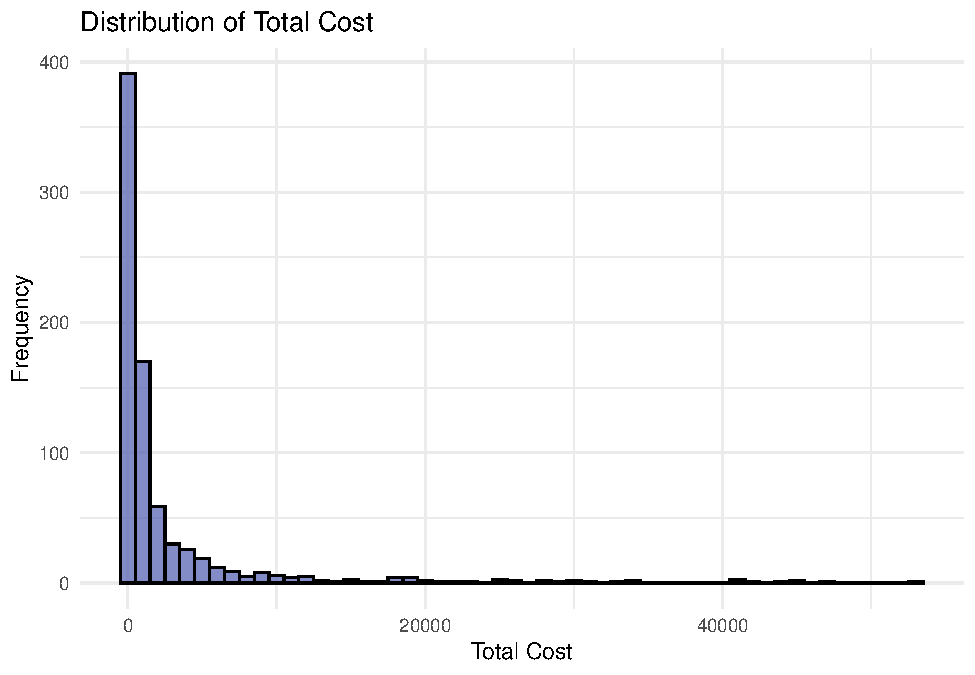
\includegraphics{p8130_hw4_xx2485_files/figure-latex/unnamed-chunk-10-1.pdf}

Apply transformations:

\begin{Shaded}
\begin{Highlighting}[]
\CommentTok{\# Apply log transformation (adding 1 to avoid log(0))}
\NormalTok{heart\_data}\SpecialCharTok{$}\NormalTok{totalcost\_log }\OtherTok{\textless{}{-}} \FunctionTok{log}\NormalTok{(heart\_data}\SpecialCharTok{$}\NormalTok{totalcost }\SpecialCharTok{+} \DecValTok{1}\NormalTok{)}

\CommentTok{\# Apply square root transformation}
\NormalTok{heart\_data}\SpecialCharTok{$}\NormalTok{totalcost\_sqrt }\OtherTok{\textless{}{-}} \FunctionTok{sqrt}\NormalTok{(heart\_data}\SpecialCharTok{$}\NormalTok{totalcost)}

\CommentTok{\# Apply inverse transformation (1/totalcost)}
\NormalTok{heart\_data}\SpecialCharTok{$}\NormalTok{totalcost\_inv }\OtherTok{\textless{}{-}} \DecValTok{1} \SpecialCharTok{/}\NormalTok{ (heart\_data}\SpecialCharTok{$}\NormalTok{totalcost }\SpecialCharTok{+} \DecValTok{1}\NormalTok{)}

\CommentTok{\# Plot transformed distributions}
\NormalTok{log\_plot }\OtherTok{\textless{}{-}} \FunctionTok{ggplot}\NormalTok{(heart\_data, }\FunctionTok{aes}\NormalTok{(}\AttributeTok{x =}\NormalTok{ totalcost\_log)) }\SpecialCharTok{+}
  \FunctionTok{geom\_histogram}\NormalTok{(}\AttributeTok{binwidth =} \FloatTok{0.5}\NormalTok{, }\AttributeTok{fill =} \StringTok{"\#1e50a2"}\NormalTok{, }\AttributeTok{color =} \StringTok{"black"}\NormalTok{, }\AttributeTok{alpha =} \FloatTok{0.7}\NormalTok{) }\SpecialCharTok{+}
  \FunctionTok{labs}\NormalTok{(}\AttributeTok{title =} \StringTok{"Log{-}Transformed Total Cost"}\NormalTok{, }\AttributeTok{x =} \StringTok{"Log(Total Cost)"}\NormalTok{, }\AttributeTok{y =} \StringTok{"Frequency"}\NormalTok{) }\SpecialCharTok{+}
  \FunctionTok{theme\_minimal}\NormalTok{()}

\NormalTok{sqrt\_plot }\OtherTok{\textless{}{-}} \FunctionTok{ggplot}\NormalTok{(heart\_data, }\FunctionTok{aes}\NormalTok{(}\AttributeTok{x =}\NormalTok{ totalcost\_sqrt)) }\SpecialCharTok{+}
  \FunctionTok{geom\_histogram}\NormalTok{(}\AttributeTok{binwidth =} \DecValTok{1}\NormalTok{, }\AttributeTok{fill =} \StringTok{"\#aacf53"}\NormalTok{, }\AttributeTok{color =} \StringTok{"black"}\NormalTok{, }\AttributeTok{alpha =} \FloatTok{0.7}\NormalTok{) }\SpecialCharTok{+}
  \FunctionTok{labs}\NormalTok{(}\AttributeTok{title =} \StringTok{"Square Root{-}Transformed Total Cost"}\NormalTok{, }\AttributeTok{x =} \StringTok{"Square Root(Total Cost)"}\NormalTok{, }\AttributeTok{y =} \StringTok{"Frequency"}\NormalTok{) }\SpecialCharTok{+}
  \FunctionTok{theme\_minimal}\NormalTok{()}

\NormalTok{inv\_plot }\OtherTok{\textless{}{-}} \FunctionTok{ggplot}\NormalTok{(heart\_data, }\FunctionTok{aes}\NormalTok{(}\AttributeTok{x =}\NormalTok{ totalcost\_inv)) }\SpecialCharTok{+}
  \FunctionTok{geom\_histogram}\NormalTok{(}\AttributeTok{binwidth =} \FloatTok{0.001}\NormalTok{, }\AttributeTok{fill =} \StringTok{"\#a22041"}\NormalTok{, }\AttributeTok{color =} \StringTok{"black"}\NormalTok{, }\AttributeTok{alpha =} \FloatTok{0.7}\NormalTok{) }\SpecialCharTok{+}
  \FunctionTok{labs}\NormalTok{(}\AttributeTok{title =} \StringTok{"Inverse{-}Transformed Total Cost"}\NormalTok{, }\AttributeTok{x =} \StringTok{"Inverse(Total Cost)"}\NormalTok{, }\AttributeTok{y =} \StringTok{"Frequency"}\NormalTok{) }\SpecialCharTok{+}
  \FunctionTok{theme\_minimal}\NormalTok{()}

\CommentTok{\# Display all plots}
\NormalTok{log\_plot}
\end{Highlighting}
\end{Shaded}

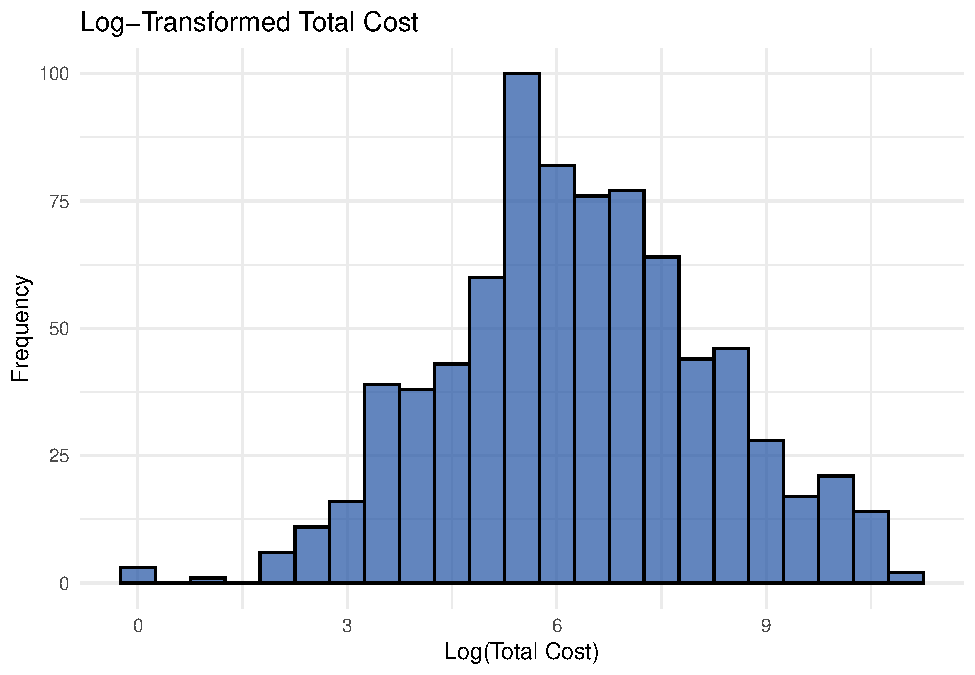
\includegraphics{p8130_hw4_xx2485_files/figure-latex/unnamed-chunk-11-1.pdf}

\begin{Shaded}
\begin{Highlighting}[]
\NormalTok{sqrt\_plot}
\end{Highlighting}
\end{Shaded}

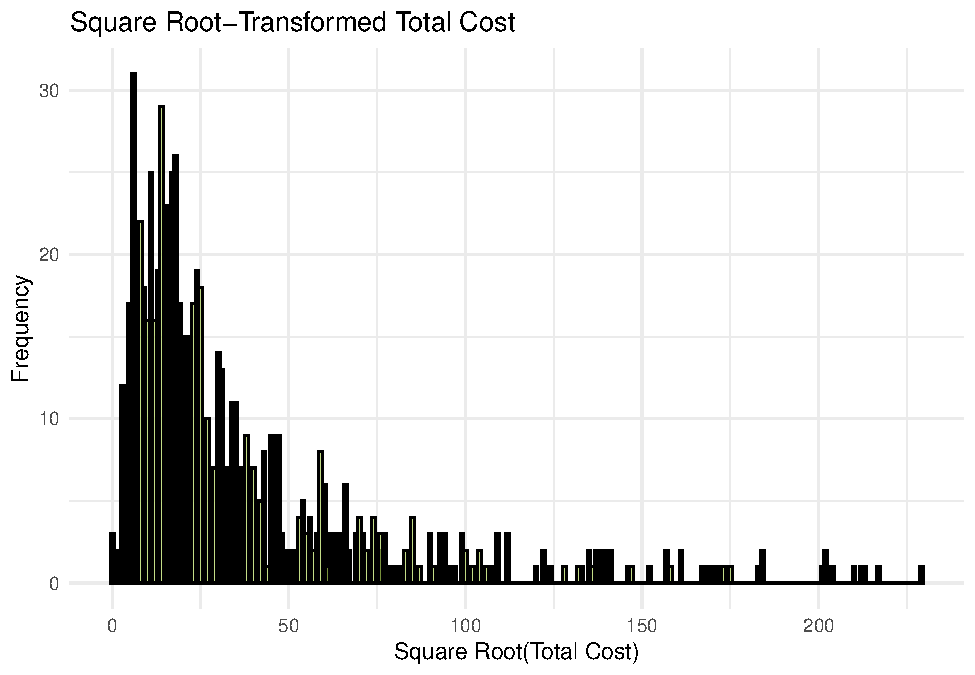
\includegraphics{p8130_hw4_xx2485_files/figure-latex/unnamed-chunk-11-2.pdf}

\begin{Shaded}
\begin{Highlighting}[]
\NormalTok{inv\_plot}
\end{Highlighting}
\end{Shaded}

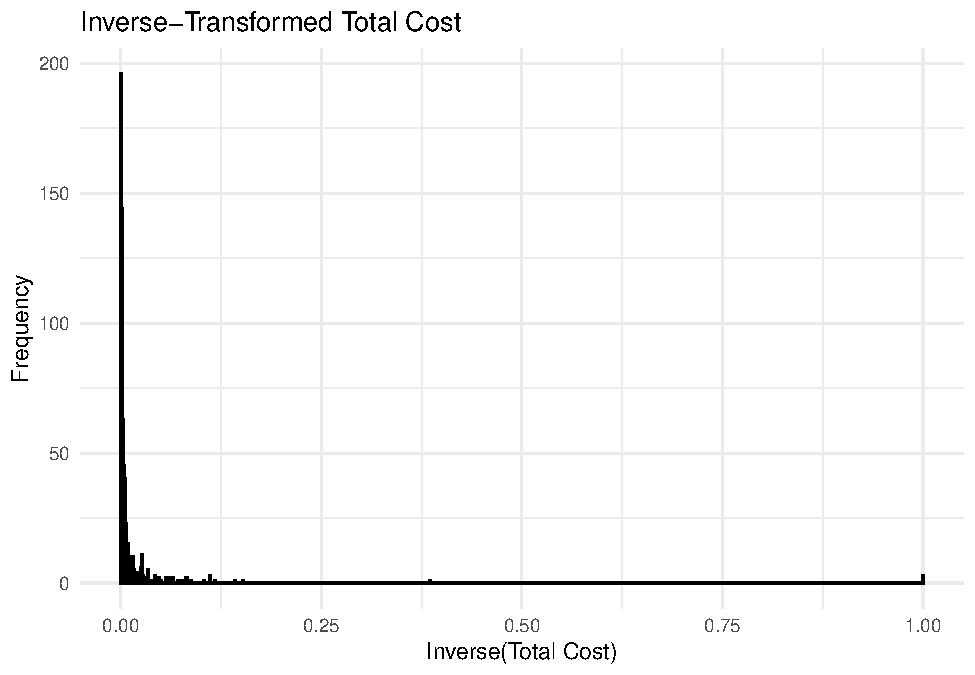
\includegraphics{p8130_hw4_xx2485_files/figure-latex/unnamed-chunk-11-3.pdf}

The shape of the distribution for variable \texttt{totalcost} is
extremely right-skewed, but after log transformation, it follows roughly
a normal distribution shape.

\subsubsection{(c)}\label{c-1}

\begin{Shaded}
\begin{Highlighting}[]
\NormalTok{heart\_data }\OtherTok{\textless{}{-}}\NormalTok{ heart\_data }\SpecialCharTok{\%\textgreater{}\%}
  \FunctionTok{mutate}\NormalTok{(}\AttributeTok{comp\_bin =} \FunctionTok{ifelse}\NormalTok{(complications }\SpecialCharTok{==} \DecValTok{0}\NormalTok{, }\DecValTok{0}\NormalTok{, }\DecValTok{1}\NormalTok{))}
\end{Highlighting}
\end{Shaded}

\subsubsection{(d)}\label{d-1}

\begin{Shaded}
\begin{Highlighting}[]
\CommentTok{\# Create scatterplot with regression line}
\FunctionTok{ggplot}\NormalTok{(heart\_data, }\FunctionTok{aes}\NormalTok{(}\AttributeTok{x =}\NormalTok{ ERvisits, }\AttributeTok{y =} \FunctionTok{log}\NormalTok{(totalcost))) }\SpecialCharTok{+}
  \FunctionTok{geom\_point}\NormalTok{(}\AttributeTok{color =} \StringTok{"\#4d5aaf"}\NormalTok{, }\AttributeTok{size =} \DecValTok{2}\NormalTok{, }\AttributeTok{alpha =} \FloatTok{0.7}\NormalTok{) }\SpecialCharTok{+}
  \FunctionTok{geom\_smooth}\NormalTok{(}\AttributeTok{method =} \StringTok{"lm"}\NormalTok{, }\AttributeTok{color =} \StringTok{"\#a22041"}\NormalTok{, }\AttributeTok{se =} \ConstantTok{TRUE}\NormalTok{) }\SpecialCharTok{+}
  \FunctionTok{labs}\NormalTok{(}\AttributeTok{title =} \StringTok{"Scatterplot of Log(Total Cost) vs ER Visits"}\NormalTok{,}
       \AttributeTok{x =} \StringTok{"Number of ER Visits"}\NormalTok{,}
       \AttributeTok{y =} \StringTok{"Log(Total Cost)"}\NormalTok{) }\SpecialCharTok{+}
  \FunctionTok{theme\_minimal}\NormalTok{()}
\end{Highlighting}
\end{Shaded}

\begin{verbatim}
## `geom_smooth()` using formula = 'y ~ x'
\end{verbatim}

\begin{verbatim}
## Warning: Removed 3 rows containing non-finite outside the scale range
## (`stat_smooth()`).
\end{verbatim}

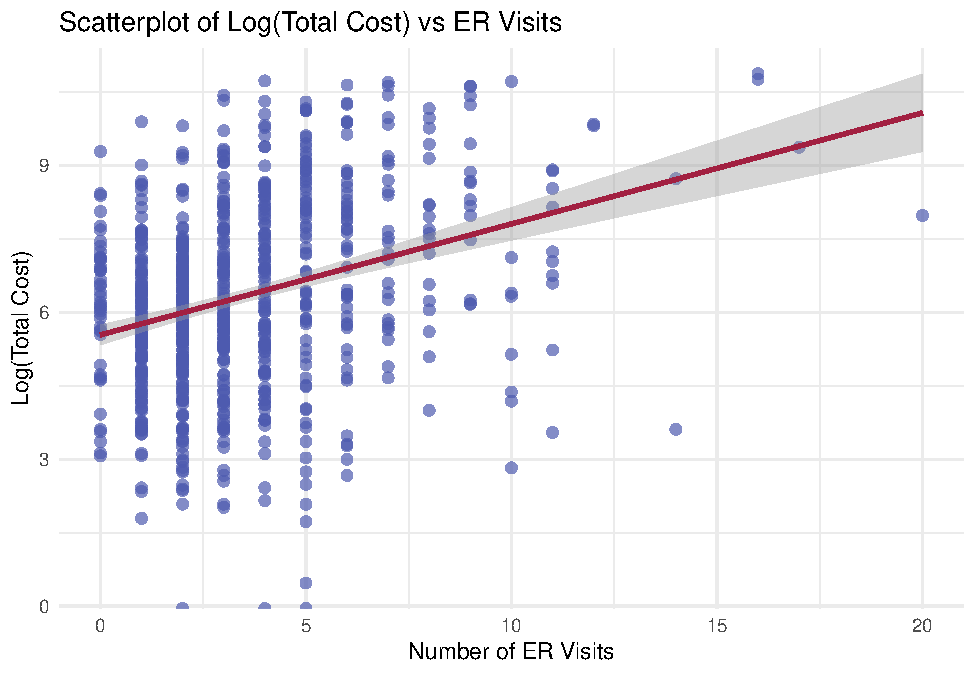
\includegraphics{p8130_hw4_xx2485_files/figure-latex/unnamed-chunk-13-1.pdf}

\begin{Shaded}
\begin{Highlighting}[]
\CommentTok{\# Fit a simple linear regression model}
\NormalTok{log\_model }\OtherTok{\textless{}{-}} \FunctionTok{lm}\NormalTok{(}\FunctionTok{log}\NormalTok{(totalcost }\SpecialCharTok{+} \DecValTok{1}\NormalTok{) }\SpecialCharTok{\textasciitilde{}}\NormalTok{ ERvisits, }\AttributeTok{data =}\NormalTok{ heart\_data)}


\CommentTok{\# Summary of regression results}
\NormalTok{model\_summary }\OtherTok{\textless{}{-}} \FunctionTok{summary}\NormalTok{(log\_model)}
\end{Highlighting}
\end{Shaded}

The p-value for the slope coefficient of \texttt{ERvisits} is
\ensuremath{1.842\times 10^{-19}}, which is less than the significance
level of 0.05. This indicates that the slope is statistically
significant. Therefore, there is strong evidence that the number of ER
visits is associated with the log-transformed total cost.

The regression equation based on the output is: \[
\text{Log(Total Cost + 1)} = 5.527 + 0.2253 \cdot \text{ERvisits}
\]

The slope coefficient for \texttt{ERvisits} is 0.2253. This means that
for every additional ER visit, the log-transformed total cost is
expected to increase by approximately 0.2253 units on average.

\subsubsection{(e)}\label{e-1}

\begin{Shaded}
\begin{Highlighting}[]
\CommentTok{\# Fit the multiple linear regression model}
\NormalTok{mlr\_model }\OtherTok{\textless{}{-}} \FunctionTok{lm}\NormalTok{(}\AttributeTok{formula =} \FunctionTok{log}\NormalTok{(heart\_data}\SpecialCharTok{$}\NormalTok{totalcost }\SpecialCharTok{+} \DecValTok{1}\NormalTok{) }\SpecialCharTok{\textasciitilde{}}\NormalTok{ heart\_data}\SpecialCharTok{$}\NormalTok{ERvisits }\SpecialCharTok{*}\NormalTok{ heart\_data}\SpecialCharTok{$}\NormalTok{comp\_bin)}

\NormalTok{mlr\_model}
\end{Highlighting}
\end{Shaded}

\begin{verbatim}
## 
## Call:
## lm(formula = log(heart_data$totalcost + 1) ~ heart_data$ERvisits * 
##     heart_data$comp_bin)
## 
## Coefficients:
##                             (Intercept)  
##                                 5.48849  
##                     heart_data$ERvisits  
##                                 0.20947  
##                     heart_data$comp_bin  
##                                 2.19096  
## heart_data$ERvisits:heart_data$comp_bin  
##                                -0.09753
\end{verbatim}

From the regression model, the interaction term
\texttt{heart\_data\$ERvisits:heart\_data\$comp\_bin} has a coefficient
of -0.09753 and a p-value of 0.311.

The p-value is greater than 0.05, indicating that the interaction term
is not statistically significant. Thus, \texttt{comp\_bin} does not
modify the relationship between \texttt{totalcost} and
\texttt{ERvisits}.

Test if comp\_bin is a confounder of the relationship between totalcost
and ERvisits.

\begin{Shaded}
\begin{Highlighting}[]
\CommentTok{\# Model 1: Without \textasciigrave{}comp\_bin\textasciigrave{}}
\NormalTok{model\_no\_comp }\OtherTok{\textless{}{-}} \FunctionTok{lm}\NormalTok{(}\FunctionTok{log}\NormalTok{(heart\_data}\SpecialCharTok{$}\NormalTok{totalcost }\SpecialCharTok{+} \DecValTok{1}\NormalTok{) }\SpecialCharTok{\textasciitilde{}}\NormalTok{ heart\_data}\SpecialCharTok{$}\NormalTok{ERvisits, }\AttributeTok{data =}\NormalTok{ heart\_data)}

\CommentTok{\# Model 2: Including \textasciigrave{}comp\_bin\textasciigrave{}}
\NormalTok{model\_with\_comp }\OtherTok{\textless{}{-}} \FunctionTok{lm}\NormalTok{(}\FunctionTok{log}\NormalTok{(heart\_data}\SpecialCharTok{$}\NormalTok{totalcost }\SpecialCharTok{+} \DecValTok{1}\NormalTok{) }\SpecialCharTok{\textasciitilde{}}\NormalTok{ heart\_data}\SpecialCharTok{$}\NormalTok{ERvisits }\SpecialCharTok{+}\NormalTok{ heart\_data}\SpecialCharTok{$}\NormalTok{comp\_bin, }\AttributeTok{data =}\NormalTok{ heart\_data)}

\CommentTok{\# Summaries of the models}
\NormalTok{summary\_no\_comp }\OtherTok{\textless{}{-}} \FunctionTok{summary}\NormalTok{(model\_no\_comp)}
\NormalTok{summary\_no\_comp}
\end{Highlighting}
\end{Shaded}

\begin{verbatim}
## 
## Call:
## lm(formula = log(heart_data$totalcost + 1) ~ heart_data$ERvisits, 
##     data = heart_data)
## 
## Residuals:
##     Min      1Q  Median      3Q     Max 
## -6.6532 -1.1230  0.0309  1.2797  4.2964 
## 
## Coefficients:
##                     Estimate Std. Error t value Pr(>|t|)    
## (Intercept)          5.52674    0.10510  52.584   <2e-16 ***
## heart_data$ERvisits  0.22529    0.02432   9.264   <2e-16 ***
## ---
## Signif. codes:  0 '***' 0.001 '**' 0.01 '*' 0.05 '.' 0.1 ' ' 1
## 
## Residual standard error: 1.799 on 786 degrees of freedom
## Multiple R-squared:  0.09844,    Adjusted R-squared:  0.09729 
## F-statistic: 85.82 on 1 and 786 DF,  p-value: < 2.2e-16
\end{verbatim}

\begin{Shaded}
\begin{Highlighting}[]
\NormalTok{summary\_with\_comp }\OtherTok{\textless{}{-}} \FunctionTok{summary}\NormalTok{(model\_with\_comp)}
\NormalTok{summary\_with\_comp}
\end{Highlighting}
\end{Shaded}

\begin{verbatim}
## 
## Call:
## lm(formula = log(heart_data$totalcost + 1) ~ heart_data$ERvisits + 
##     heart_data$comp_bin, data = heart_data)
## 
## Residuals:
##     Min      1Q  Median      3Q     Max 
## -6.5249 -1.0769 -0.0074  1.1847  4.4024 
## 
## Coefficients:
##                     Estimate Std. Error t value Pr(>|t|)    
## (Intercept)          5.51020    0.10279  53.606  < 2e-16 ***
## heart_data$ERvisits  0.20295    0.02405   8.437  < 2e-16 ***
## heart_data$comp_bin  1.70573    0.27915   6.111 1.56e-09 ***
## ---
## Signif. codes:  0 '***' 0.001 '**' 0.01 '*' 0.05 '.' 0.1 ' ' 1
## 
## Residual standard error: 1.759 on 785 degrees of freedom
## Multiple R-squared:  0.1394, Adjusted R-squared:  0.1372 
## F-statistic: 63.57 on 2 and 785 DF,  p-value: < 2.2e-16
\end{verbatim}

Compare the coefficients.

\begin{Shaded}
\begin{Highlighting}[]
\CommentTok{\# Extract coefficients for \textasciigrave{}ERvisits\textasciigrave{}}
\NormalTok{coef\_no\_comp }\OtherTok{\textless{}{-}}\NormalTok{ summary\_no\_comp}\SpecialCharTok{$}\NormalTok{coefficients[}\StringTok{"heart\_data$ERvisits"}\NormalTok{, }\StringTok{"Estimate"}\NormalTok{]}
\NormalTok{coef\_with\_comp }\OtherTok{\textless{}{-}}\NormalTok{ summary\_with\_comp}\SpecialCharTok{$}\NormalTok{coefficients[}\StringTok{"heart\_data$ERvisits"}\NormalTok{, }\StringTok{"Estimate"}\NormalTok{]}

\CommentTok{\# Calculate percent change}
\NormalTok{percent\_change }\OtherTok{\textless{}{-}} \FunctionTok{abs}\NormalTok{((coef\_with\_comp }\SpecialCharTok{{-}}\NormalTok{ coef\_no\_comp) }\SpecialCharTok{/}\NormalTok{ coef\_no\_comp) }\SpecialCharTok{*} \DecValTok{100}

\CommentTok{\# Display results}
\FunctionTok{cat}\NormalTok{(}\StringTok{"Coefficient of ERvisits without comp\_bin:"}\NormalTok{, }\FunctionTok{round}\NormalTok{(coef\_no\_comp, }\DecValTok{4}\NormalTok{), }\StringTok{"}\SpecialCharTok{\textbackslash{}n}\StringTok{"}\NormalTok{)}
\end{Highlighting}
\end{Shaded}

\begin{verbatim}
## Coefficient of ERvisits without comp_bin: 0.2253
\end{verbatim}

\begin{Shaded}
\begin{Highlighting}[]
\FunctionTok{cat}\NormalTok{(}\StringTok{"Coefficient of ERvisits with comp\_bin:"}\NormalTok{, }\FunctionTok{round}\NormalTok{(coef\_with\_comp, }\DecValTok{4}\NormalTok{), }\StringTok{"}\SpecialCharTok{\textbackslash{}n}\StringTok{"}\NormalTok{)}
\end{Highlighting}
\end{Shaded}

\begin{verbatim}
## Coefficient of ERvisits with comp_bin: 0.2029
\end{verbatim}

\begin{Shaded}
\begin{Highlighting}[]
\FunctionTok{cat}\NormalTok{(}\StringTok{"Percent change in coefficient:"}\NormalTok{, }\FunctionTok{round}\NormalTok{(percent\_change, }\DecValTok{2}\NormalTok{), }\StringTok{"\%}\SpecialCharTok{\textbackslash{}n}\StringTok{"}\NormalTok{)}
\end{Highlighting}
\end{Shaded}

\begin{verbatim}
## Percent change in coefficient: 9.92 %
\end{verbatim}

Conclusion: The percent change in the coefficient of ERvisits is less
than 10\% (9.92\%). This suggests that comp\_bin is not a significant
confounder of the relationship between totalcost and ERvisits.

\texttt{comp\_bin} should be included along with \texttt{ERvisits}.
\texttt{comp\_bin} is a statistically significant predictor, so it
improves the explanatory power of the model. It does not act as a
confounder either.

Adding \texttt{comp\_bi}n provides additional information about
\texttt{totalcost} without distorting the relationship between
\texttt{ERvisits} and \texttt{totalcost}.

\subsubsection{(f)}\label{f}

\begin{Shaded}
\begin{Highlighting}[]
\CommentTok{\# Fit the MLR model with additional covariates}
\NormalTok{mlr\_model\_extended }\OtherTok{\textless{}{-}} \FunctionTok{lm}\NormalTok{(}\FunctionTok{log}\NormalTok{(totalcost }\SpecialCharTok{+} \DecValTok{1}\NormalTok{) }\SpecialCharTok{\textasciitilde{}}\NormalTok{ ERvisits }\SpecialCharTok{+}\NormalTok{ comp\_bin }\SpecialCharTok{+}\NormalTok{ age }\SpecialCharTok{+}\NormalTok{ gender }\SpecialCharTok{+}\NormalTok{ duration, }\AttributeTok{data =}\NormalTok{ heart\_data)}

\CommentTok{\# Show the regression results}
\FunctionTok{summary}\NormalTok{(mlr\_model\_extended)}
\end{Highlighting}
\end{Shaded}

\begin{verbatim}
## 
## Call:
## lm(formula = log(totalcost + 1) ~ ERvisits + comp_bin + age + 
##     gender + duration, data = heart_data)
## 
## Residuals:
##     Min      1Q  Median      3Q     Max 
## -5.4711 -1.0340 -0.1158  0.9493  4.3372 
## 
## Coefficients:
##                Estimate Std. Error t value Pr(>|t|)    
## (Intercept)   5.9404610  0.5104064  11.639  < 2e-16 ***
## ERvisits      0.1745975  0.0225736   7.735 3.20e-14 ***
## comp_bin      1.5044946  0.2584882   5.820 8.57e-09 ***
## age          -0.0206475  0.0086746  -2.380   0.0175 *  
## genderFemale -0.2067662  0.1387002  -1.491   0.1364    
## duration      0.0057150  0.0004888  11.691  < 2e-16 ***
## ---
## Signif. codes:  0 '***' 0.001 '**' 0.01 '*' 0.05 '.' 0.1 ' ' 1
## 
## Residual standard error: 1.624 on 782 degrees of freedom
## Multiple R-squared:  0.2694, Adjusted R-squared:  0.2647 
## F-statistic: 57.68 on 5 and 782 DF,  p-value: < 2.2e-16
\end{verbatim}

F-statistic and overall significance:

\begin{itemize}
\item
  The overall F-statistic is 57.68, with a p-value of 782
  (\(p < 0.05\)).
\item
  This shows that the model is statistically significant and that the
  predictors collectively explain variability in log-transformed total
  cost.
\end{itemize}

Comments on Individual Predictors

\begin{enumerate}
\def\labelenumi{\arabic{enumi}.}
\item
  ERvisits:

  \begin{itemize}
  \item
    Coefficient: 0.1746
  \item
    \(p\)-value: \ensuremath{3.197\times 10^{-14}}
  \item
    Interpretation: ER visits are significantly increase log-transformed
    total cost (\(p < 0.05\)).
  \end{itemize}
\item
  comp\_bin:

  \begin{itemize}
  \item
    Coefficient: 1.504
  \item
    \(p\)-value: \ensuremath{8.566\times 10^{-9}}
  \item
    Interpretation: Complications significantly increase log-transformed
    total cost (\(p < 0.05\)).
  \end{itemize}
\item
  age:

  \begin{itemize}
  \item
    Coefficient: -0.02065
  \item
    \(p\)-value: 0.01754
  \item
    Interpretation: Age significantly increase log-transformed total
    cost (\(p < 0.05\)).
  \end{itemize}
\item
  gender:

  \begin{itemize}
  \item
    Coefficient: -0.2068
  \item
    \(p\)-value: 0.1364
  \item
    Interpretation: Gender is not statistically significant
    (\(p = 0.1364\)).
  \end{itemize}
\item
  duration:

  \begin{itemize}
  \item
    Coefficient: 0.005715
  \item
    \(p\)-value: \ensuremath{3.258\times 10^{-29}}
  \item
    Interpretation: Duration significantly increase log-transformed
    total cost (\(p < 0.05\)).
  \end{itemize}
\end{enumerate}

The model explains approximately 27\% of the variability in
log-transformed total cost. \texttt{ERvisits}, \texttt{comp\_bin},
\texttt{age}, and \texttt{duration} are statistically significant, while
\texttt{gender} is not. Duration has the strongest positive association
with log-transformed total cost, followed by \texttt{comp\_bin} and
\texttt{ERvisits}.

Compare the SLR and MLR models.

Key Metrics from SLR Model

\begin{enumerate}
\def\labelenumi{\arabic{enumi}.}
\item
  Residual Standard Error: 1.799
\item
  \(R^2\): 0.09844 (approximately 9.8\% of variability in total cost
  explained by ER visits alone).
\item
  ERvisits Coefficient:

  \begin{itemize}
  \tightlist
  \item
    Estimate: 0.2253
  \item
    \(p\)-value: \ensuremath{1.842\times 10^{-19}}
  \item
    Interpretation: The SLR model shows a statistically significant
    positive association between ER visits and total cost
    (\(p < 0.05\)).
  \end{itemize}
\end{enumerate}

Key Metrics from MLR Model

\begin{enumerate}
\def\labelenumi{\arabic{enumi}.}
\item
  Residual Standard Error: 1.624
\item
  \(R^2\): 0.2694 (approximately 27\% of variability in total cost
  explained by ER visits along with other predictors).
\item
  Adjusted \(R^2\): 0.2647.
\item
  ERvisits Coefficient:

  \begin{itemize}
  \tightlist
  \item
    Estimate: 0.1746
  \item
    \(p\)-value: \ensuremath{3.197\times 10^{-14}}
  \item
    Interpretation: Even after adjusting for \texttt{comp\_bin},
    \texttt{age}, \texttt{gender}, and \texttt{duration}, ER visits
    remain a statistically significant positive predictor of total cost
    (\(p < 0.05\)).
  \end{itemize}
\end{enumerate}

Since the investigator's primary objective is the association between
total cost and ER visits, the \textbf{SLR model} would be used to
address the objective. It directly quantifies the relationship without
adjusting for additional variables, making it simpler and more
interpretable for this specific research question. However, if
confounders like \texttt{comp\_bin} are taken into consideration, the
\textbf{MLR model} would be more appropriate.

\end{document}
